\documentclass[a4paper]{article}

\usepackage{geometry}
\usepackage{natbib}
\bibpunct[:]{(}{)}{,}{a}{}{;}

%--------------------
%\usepackage{gb4e}
%\noautomath

\usepackage{amsmath}
\usepackage{amsfonts}
\usepackage{amsthm}
\usepackage{amssymb}
\usepackage{mathrsfs}
\usepackage{nicefrac}
%\usepackage{stmaryrd}
%\usepackage{multicol}
\usepackage{graphicx}
\usepackage{color}
%\newcommand{\mvalueof}[1]{\llbracket#1\rrbracket}
\newcommand{\citeposs}[2][]{\citeauthor{#2}'s (\citeyear[#1]{#2})}
\newcommand{\tuple}[1]{\ensuremath{\left\langle #1 \right\rangle}} 

\newcommand{\hl}[1]{\textcolor[rgb]{.8,.33,.0}{#1}}% prints in orange
%\newcommand{\argmax}[1]{\underset{#1}{\operatorname{arg}\,\operatorname{max}}\;}
%\newcommand{\argmin}[1]{\underset{#1}{\operatorname{arg}\,\operatorname{min}}\;}
%\newcommand{\sbna}{\exists\lnot\forall}

%--------------------
%
%\usepackage{setspace}
%\onehalfspacing
%
%-------------------


\title{Communicative pressures at the semantics-pragmatics interface:\\ Learning biases may prevent the lexicalization of pragmatic inferences}

\author{%\bf NAME1 and NAME2\\
    ( -- draft \today --- )
}


\date{}

\begin{document}
\maketitle

\begin{abstract} Certain classes of lexical meanings enable for pragmatic enrichments in a notably productive fashion. This raises the challenge to justify their regular selection over alternatives that codify semantically what is conveyed pragmatically. To address this issue, we propose a general model that integrates iterated Bayesian learning in the replicator-mutator dynamics. This model generates predictions about the effects of linguistic pressures on selection and transmission in populations of probabilistic language users with varied degrees of pragmatic sophistication. We apply this model in a case study on the (lack of) lexicalization of scalar implicatures. The results show that simpler semantic representations are selected for when languages are pressured towards learnability and compression, provided that pragmatic reasoning can compensate for the disadvantage in expressivity that users of such languages otherwise incur. We argue this result to shed light on the lack of lexicalization of scalar inferences, as well as the semantics-pragmatics distinction more generally.
\end{abstract}

\section{Simplicity, expressivity, and learnability at the semantics-pragmatics interface}\label{sec:introduction}


In linguistic theorizing it is common to draw a distinction between semantics and pragmatics. Broadly speaking, the former concerns the truth-conditional content of expressions whereas the latter concerns information beyond literal meanings and their composition. An important consequence of this distinction is that the information conveyed by an utterance is seldom, if ever, solely determined by semantics, but rather in tandem with pragmatics. Much research at the semantics-pragmatics interface has been aimed at characterizing expressions in terms of either domain or their interplay. However, an issue that has received little attention is the justification of semantic structure in light of pragmatics. The present investigation seeks to fill this gap by analyzing the effects linguistic pressures have on the selection and pervasiveness of particular lexical meanings under consideration of their possible pragmatic enrichments.

In recent years questions about the emergence and stability of linguistic features have lead to a surge in models that analyze their transmission within and across generations (see \citealt{steels:2015} and \citealt{tamariz+kirby:2016} for recent overviews). Our starting point is given by the overarching argument that has crystalized from the accumulated mathematical, experimental and cross-linguistic evidence in this literature: Natural languages need to be well-adapted to communicative needs within a linguistic community, but also need to be learnable to survive their faithful transmission across generations. More succinctly; natural languages are pressured for expressivity and learnability.   

We build on these insights by modeling these pressures using the replicator-mutator dynamics (see \citealt{hofbauer+sigmund:2003} for an overview). This allows for the inspection of their interaction by combining functional pressure on successful communication with effects of learning biases on (iterated) Bayesian learning \citep{griffiths+kalish:2007}. The semantics-pragmatics distinction and its effect on production and comprehension are made precise by considering probabilistic models of rational language use in populations with distinct lexica \citep{frank+goodman:2012,franke+jaeger:2014, bergen+etal:2016}. \hl{SOMETHING MISSING HERE} \hl{In this way, the model establishes a link between models of synchronic probabilistic rational language use and diachronic models of cultural evolution. }

%We then analyze the prevalence of a lack of semantic upper-bounds in the literal meaning of weak scalar expressions. We show that a lack of upper-bounds is selected for when learners are biased towards simpler semantic representations, provided they have means to convey upper-bounds, i.e., provided that they can be derived via pragmatic reasoning.  

The emergence and change of linguistic structure is influenced by many intertwined factors. These range from biological and socio-ecological to cultural \citep{steels:2011,tamariz+kirby:2016}. Social and ecological pressures determine communicative needs, while biology determines the architecture that enables and constrains the means by which they can be fulfilled. Our focus lies on the latter, cultural, factor wherein processes of linguistic change are understood as shaped by language use and its transmission. That is, as a result of a process of cultural evolution.

At latest since \citeposs{zipf:1949} rationalization of the observation that word frequency rankings can be approximated by a power law distribution as competing hearer and speaker preferences, the idea that linguistic change is influenced by communicative pressures has played a pivotal role in synchronic and diachronic analyses (e.g. \citealt{martinet:1962, horn:1984,jaeger+vRooij:2007,jaeger:2007, piantadosi:2014,kirby+etal:2015}). 

As noted above, expressivity and learnability have been identified as two central competing pressures. Their opposition becomes particularly clear when considering their consequences in the extreme (cf. \citealt{kemp+regier:2012,kirby+etal:2015}). On one extreme, a language with a single form is easy to learn but lacking in expressivity. On the other, a language that associates a distinct form with all possible meanings its users may want to convey is maximally expressive but challenging to acquire. The most prominent problem that arises from this tension is that of acquiring a language to express a potentially infinite set of meanings through finite means \citep{kirby:2002}. However, this so-called transmission bottleneck is not the only challenge learners confront. Instead, a problem that is more important for our present purpose is that of selecting particular hypotheses out of a (potentially infinite) space of alternatives compatible with the data learners are exposed to. At the semantics-pragmatics interface this concerns the selection between functionally similar, if not identical, lexical meanings.  In the following, we argue an integral part of the answer to be that learners are a priori biased towards simpler, more compressed, lexical representations. That is, rational learners should prefer simpler over more complex explanations of the data they witness \citep{feldman:2000, chater+vitanyi:2003, piantadosi+etal:2012a, kirby+etal:2015,piantadosi+etal:underreview}. In linguistics, a drive for simplicity has been argued to underpin speaker preferences for brevity and ease of articulation, as well as to pressure languages towards lexical ambiguity and grammatical compression \citep{zipf:1949,grice:1975,piantadosi+etal:2012, kirby+etal:2015}. \hl{As a broader cognitive principle, the use of simplicity as means to select between hypotheses has a long standing tradition. Crucially, \citet{chater+vitanyi:2003} give a number of compelling arguments for simplicity on both mathematical and empirical grounds.}


The remainder of this section introduces the individual components of the model in more detail, as well as the assumptions underlying them. These are: (i) the representation of languages and their use, (ii) pressures towards expressivity and learnability, regulated by the replicator and mutator dynamics, respectively, as well as (iii) a bias towards simpler semantic representations, codified as a language learner's prior. After laying out the model, we discuss its application to the lack of lexicalization of scalar implicatures.




\subsection{Lexica and linguistic behavior}
Lexica codify the truth-conditions of a language's expressions, i.e., its semantics. A convenient way to represent them is by $(|S|,|M|)$-Boolean matrices, where $S$ is a set of states of affairs -- or meanings -- to convey and $M$ a set of messages of the language \citep{franke+jaeger:2014}. For example, the following two fragments determine the truth-conditions of two messages, $m_1$ and $m_2$, for two states, $s_1$ and $s_2$.

\begin{centering}
$L_a$ = \bordermatrix{~ & m_1 & m_2 \cr 
                  s_1 & 1 & 0 \cr
                  s_2 & 1 & 1 \cr} \hspace{2cm} $L_b$ = \bordermatrix{~ & m_1 & m_2 \cr 
                  s_1 & 1 & 0 \cr
                  s_2 & 0 & 1 \cr}\\[0.5cm]
\end{centering}


According to lexicon $L_a$ the message $m_1$ is true of state $s_1$ as well as of $s_2$. In contrast, $m_1$ is only true of $s_1$ in $L_b$. Otherwise, the two languages are truth-conditionally equivalent. 

To make the distinction betweeen semantics and pragmatics precise, we distinguish between two kinds of linguistic behavior. {\em Literal interlocutors} produce and interpret messages literally. That is, their linguistic choices are guided only by their lexica. In contrast, {\em pragmatic interlocutors} engage in mutual reasoning to inform their choices. For instance, a rational speaker of $L_a$ who reasons about her addressee may use $m_1$ to exclusively signal state $s_1$ given that $s_2$ can unambiguously be conveyed through $m_2$. Accordingly, rational hearers that expect their interlocutor to reason along these lines will interpret ambiguous $m_1$ as $s_1$. An important consequence of this pragmatic process is that it renders $L_a$ indistinguishable from $L_b$ in terms of expressivity. 

Following models of rational language use such as Rational Speech Act models \citep{frank+goodman:2012} and their game-theoretic counterparts \citep{benz+etal:2005a,franke:2009,franke+jaeger:2014}, this kind of signaling behavior is captured by a resaoning hierarchy. The hierarchy's bottom, level $0$, corresponds to literal language use. Pragmatic language users of level $n + 1$ behave rationally according to (expected) level $n$ behavior of their interlocutors. (\ref{h:level0}) and (\ref{h:leveln}) specify the behavior of literal and pragmatic hearers of a language $L$. Mutatis mutandis for the literal and pragmatic speakers in (\ref{s:level0}) and (\ref{s:leveln}).

\begin{flalign}
&H_{0}(s|m;L) \propto pr(s) L_{sm} \label{h:level0}\\
&S_{0}(m|s;L) \propto \exp(\lambda \; L_{sm}) \label{s:level0}\\
&H_{n+1}(s|m;L) \propto pr(s) S_{n}(m|s;L) \label{h:leveln}\\
&S_{n+1}(m|s;L) \propto  \exp(\lambda \; H_{n}(s|m;L)^\alpha) \label{s:leveln}
\end{flalign}

According to (\ref{h:level0}) a literal hearer's interpretation of a message $m$ as a state $s$ depends on her lexicon and her prior over states, $pr \in \Delta(S)$. The literal speaker's behavior as given in (\ref{s:level0}) is regulated by a soft-max parameter $\lambda$, $\lambda \geq 1$ \citep{luce:1959,sutton+barto:1998}. As $\lambda$ increases, choices made in production are more rational. That is, higher values lead to behavior that is increasingly in line with expected utility maximization. 

Pragmatic behavior is similar to its literal counterpart. As in our informal sketch, their difference lies in that level $n+1$ speakers/hearers reason about level $n$ hearer/speaker behavior instead of solely relaying on their lexicon. That is, they reason about how a rational level $n$ interlocutor would use or interpret a message, and behave according to these expectations. Pragmatic production is further regulated by a parameter $\alpha$ which controls the tension between semantics and pragmatics, $\alpha \in (0,1]$. Lower values lead to more literal production whereas higher values lead to stronger pragmatic behavior. 

The combination of a lexicon with its use, i.e., a level in the reasoning hierarchy, is called a type. These are the basic units on which our population dynamics operate. 

\subsection{Replication \& expressivity}
Communicative efficiency, or expressivity, has received particular attention from investigations using evolutionary game theory \citep{nowak+krakauer:1999,nowak+etal:2000, nowak+etal:2002}. Under this view, a type's success in communication confers it a higher fitness relative to less successful ones. As a consequence they replicate more than other types, increasing their proportion in the population. This association of a type's communicative success within a population with changes in the types present in it creates a feedback loop that pressures the population towards greater expressivity. The replicator equation gives us the means to make these dynamics precise.

The proportion of types in a given population is captured by a vector $x$, where $x_i$ is type $i$'s proportion in the population. The fitness of a type $i$, $f_i$, is given by its expected utility in this population, $f_i = \sum_j x_j \text{EU}(t_i,t_j)$. That is, its fitness is the sum of its expected communicative success with other types weighted by the latter type's population share. The expected utility of $i$ and $j$ is obtained by considering the expected utility of speaker $i$ interacting with hearer $j$, and vice versa: $\text{EU}(t_i,t_j) = [U_S(t_i,t_j) + U_R(t_i,t_j)]/2$. $U_S(x,y)$ and $U_R(x,y)$ are respectively $\sum_s P(s)\sum_m S_n(m|s;L) \sum_{s'} R_o(s'|m;L) \delta(s,s')$ and $U_S(y,x)$ for $n$ and $o$ being the reasoning level of $x$ and $y$, and $\delta(s,s') = 1$ iff $s = s'$ and $0$ otherwise.\footnote{Note that the definition of $U_R(\cdot,\cdot)$ implies equal sender and receiver payoff in an interaction. This need not be so in the general case but suffices for our application.} This quantity is symmetric, reflecting the probability of two types' mutual understanding. Lastly, the average fitness of the population is captured by $\Phi$, $\Phi = \sum_i x_i f_i$. This term serves as a normalizing constant for the (discrete) replicator equation; $\dot{x}_i = \frac{x_i f_i}{\Phi}$ 

Under its biological interpretation, the replicator equation captures the idea of fitness-relative selection whereby fitter types produce more offspring, leading to their propagation in subsequent generations. In analogy to this kind of replication, many aspects of natural language are subject to processees of transmission and change across varied time-spans. For example, the replicator equation can be understood as a learning across generations as e.g. in \citealt{nowak+etal:2002}, but also as a process of horizontal adaptation (see \citealt[\S3.3]{benz+etal:2005b} for discussion). In the following, we take the latter view in assuming that interlocutors adapt their lexica and their use to that which works best within their population. It should be stressed, however, that the model itself is compatible with either view. 

Nowak et al. did not only consider replication, but also recognized the important role of the variation that is introduced by a language's transmition across generations, construed as mutation. Due to this process, the offspring of a type may end up adopting a different type than that of its parent. Crucially, in this work mutation rates were modelled as begin independent from a type. This means that the variation introduced by generational turnovers did not depend on factors such as the relative learnability of a type. To address the issue of selecting a particular type over (near) functional equivalents, we turn to a different strand of research in cultural evolution: {\em iterated learning}. 


\subsection{Mutation \& learning}\label{sec:mutation}
Iterated learning is a process in which the behavior of one individual serves as learning input for another, who's behavior subsequently serves as input for a new learner, and so on. For linguistic purposes this process can be thought of as chains of parents and children, where the parent produces linguistic data from which the child infers a language. The latter, now a parent, goes on to produce linguistic data for a new generation of na\"ive learners. Following \citet{griffiths+kalish:2007} we model learning as a process of Bayesian inference in which learners combine the likelihood of a type producing the learning data with prior inductive biases. They then select a type to adopt from the resulting posterior distribution.

Due to the pressure towards learnability it exherts, iterated learning generally leads to simpler and more regular languages (surveys of empirical data and models are given in \citealt{kirby+etal:2014} and \citealt{tamariz+kirby:2016}). Importantly, experimental and mathematical results suggest the results of this process to reflect learners' learning biases, codified in the following as a prior $P \in \Delta(\mathcal{T})$. A way to think about this bias is as the amount of data a learner would require in order to adopt a language -- or, in our case, a combination of a lexicon and a signaling behavior (cf. \citealt[450]{griffiths+kalish:2007}). Crucially, the extent of the prior's influence has been shown to strongly depend on the learning strategy assumed to underly the inference process. While simulation results suggested that weak biases could be magnified by exposing learners to only small data samples \citep{brighton:2002}, the mathematical characterization provided by \citet{griffiths+kalish:2007} showed that, instead, iterated learning converged to the prior. That is, the distribution over languages in a population or, from an individual's perspective, the likelihood of learning a language corresponds to the learners' prior distribution, irrespective of the amount of input given to learners. This divergence in predictions can be traced back to differences in the selection of hypotheses from the posterior. On the one extreme, Griffith \& Kalish's convergence to the prior holds for learners that sample from the posterior. On the other, more deterministic strategies such as the selection of the type with the highest posterior probability, so-called {\it maximum a posterior estimation} (MAP), increase the prior's influence \citep{griffiths+kalish:2007,kirby+etal:2007}. In the following, we parametrize the posterior, $P(t_i|d)^l$, to obtain a range of learning strategies that live in the range between posterior sampling and MAP, $l \geq 1$. When $l = 1$ learners sample from the posterior. As $l$ increases towards infinity, the learners' tendency maximize the posterior increases. 

More generally, we combine the replicator dynamics with iterated learning by codifying the latter as a transition matrix $Q$. Just as in standard mutator dynamics, $Q_{ij}$ indicates the probability of the children of a parent of type $i$ adopting type $j$. However, to make this process depend on a type's learnbility, this quantity is proportional to the probability of $i$ producing the learning data and that of $j$ given the data. 

The elements of the set of learning data $D$ are sequences of length $k$ of state-message pairings. That is, a sequence of observations of language use. Put differently, a datum $d \in D$ contains $k$ members of the set $\{\tuple{s_i,m_j} | s_i \in S, m_j \in M\}$ and $D$ is the set of all such sequences. Having fixed $D$,
\[
 Q_{ij} \propto \sum_{d \in D} P(d|t_i) F(t_j,d),
\]
where $F(t_j,d) \propto P(t_j|d)^l$ and $P(t_j|d) \propto P(t_j) P(d|t_j)$. Given a type $i$, $P(d|t_i)$ can be straightforwardly computed based on $t_i$'s production behavior. 
 

\subsection{Summary}
We argued for expressivity, learnability and simplicity as important pressures that apply on the cultural evolution of language. They are respectively modelled as communicative efficiency-relative replication, iterated Bayesian learning, and a prior that biases learners for compressed lexical meanings. Taken together these evolutionary dynamics are described by the replicator-mutator dynamics \citep{hofbauer+sigmund:2003}: 

\[ 
\hat{x_i} = \sum_j Q_{ji} \frac{x_jf_j}{\Phi}
\]

The basic units that the dynamics operate on are a combination of lexica lexicon and their use; a type. A type's expressivity depends on its communicative efficiency within a population while its learnability depends on the fidelity by which it is infered by new generations of na\"ive learners. 

In sum, the innovation of this model lies in its combination of functional pressure on successful communication, effects of learning biases on (iterated) Bayesian language learning \citealt{griffiths+kalish:2007}, and probabilistic models of language use in populations with distinct lexica \citep{frank+goodman:2012,franke+jaeger:2014,bergen+etal:2016}. In particular, this synthesis enables for the investigation of the effects of communicative pressures on the semantics-pragmatics interface. In doing so, it links the previously disconnected areas of rational probabilistic language use and cultural evoltion.

%\hl{So far, we have focused on highlighting the strands of research and assumptions present in the model. Less has been said about its departure from past approaches, beyond the virtues we argued their synthesis gives rise to. Given the different foci of these investigations, most comparisons on a general level are misplaced. However, \citet{kirby+etal:2015} ...}






%%%Differences to our earlier CogSci proceedings paper:
%Sequences and atomic observations. Before, the set of all observations was $O =$\linebreak  $\{\tuple{\tuple{s_1,m_i},\tuple{s_2,m_j}} | m_i, m_j \in M\}$. A member of $O$ encodes that a teacher produced $m_i$ in state $s_1$ and $m_j$ in $s_2$, i.e., it encodes one witnessed message for each state.

%Observations as production. Instead of taking the space of all possible sequences of length $k$ into consideration, we take sample from $O$ $k$-times according to the production probabilities of each type; $P(o = \tuple{s,m} | t_i) = P(s) P(m|s,t_i)$. $n$ such $k$-length sequences are sampled for each type. As a consequence, the data used for computing $Q_i$ is not the same as that used for $j$ $(i \neq j)$.

%No communal learniner; only parental
%%%

\section{Lack of lexicalization of pragmatic inferences}

%
With this model, we set out to investigate the prevalence of lexical meanings that allow for regular pragmatic enrichments over other alternatives. A particularly well-studied type of conventional pragmatic enrichment are so-called {\em scalar implicatures}. These inferences are licensed for groups of expressions ordered in terms of informativity, here understood as an entailment induced order. For instance, {\em some} is entailed by {\em all}; if it were true that `All students came to class', it would also be true that `Some students came to class'. However, while weaker expressions such as {\em some} are truth-conditionally compatible with stronger alternatives such as {\em all}, this is not necessarily what their use is taken to convey. Instead, the use of a less informative expression when a more informative one could have been used can license a defeasible inference that stronger alternatives do not hold (cf. \citealt{horn:1972,gazdar:1979}). That is, a hearer who assumes the speaker to be able and willing to provide all relevant information can infer that, since the speaker did not use a stronger alternative, e.g. {\em all}, this alternative must not hold. In this way, `Some students came to class' is strengthened to convey `Some but not all students came to class'. Analogously, a speaker can rely on her interlocutor to draw this inference without having to express this upper-bound overtly, e.g. by stating {\em some but not all}. In other words, mutual reasoning about rational language use supplies a bound that rules out stronger alternatives pragmatically.

This corresponds to our previous description of the pragmatic use of lexicon $L_a$, repeated below for convenience. A pragmatic hearer who reasons about a speaker's use of message $m_1$ will associate it more strongly with $s_1$ than with $s_2$ given that the latter is unambiguously associated with $s_2$. The strength of this association dependens on the individuals' degree of rationality $\lambda$ and their prior over states. Conversely, a pragmatic speaker will reason about her interlocutor's interpretation and use the messages accordingly. 

\begin{centering}
$L_a$ = \bordermatrix{~ & m_1 & m_2 \cr 
                  s_1 & 1 & 0 \cr
                  s_2 & 1 & 1 \cr} \hspace{2cm} $L_b$ = \bordermatrix{~ & m_1 & m_2 \cr 
                  s_1 & 1 & 0 \cr
                  s_2 & 0 & 1 \cr}\\[0.5cm]
\end{centering}

Our initial question can now be rephrased in terms of scalar implicatures by asking for justifiations for the lack of lexical upper-bounds in weak scalar alternatives. That is, why semantics such as those of message $m_1$ in $L_a$ are regularly selected for over the alternative of lexicalizing it as in $L_b$. More poignantly, would it not serve language users better if weak(er) expressions such as {\em warm}, {\em or}, {\em some} or {\em big} were truth-conditionally incompatible with stronger alternatives such as, respectively, {\em hot}, {\em and}, {\em all} and {\em huge}?  This question is particularly striking considering the number of expressions that license such inferences across languages (\citealt{horn:1972}, \citealt[252-267]{horn:1984}, \citealt{traugott:2004,vdAuwera:2010}). 

We see two main explanations for the lack of upper-bounds in the lexical meaning of weak scalar expressions. The first is that their truth-conditional compatibility with stronger expressions endows them a broader range of application. Scalar expressions occur in contexts in which their upper-bounded reading is absent. This can happen when embedded in downward-entailing contexts, when the speaker is likely uncertain about whether the upper bounded reading is true, or when the distinction between an upper-bounded reading and the simple, only lower-bounded reading, is not relevant. For instance, if for all the speaker knows `Some students came' but she doesn't know whether `All came', then the use of {\em some} succinctly conveys her uncertainty about the latter. This may suggest a functionalist argument for why upper-bounded meanings do not conventionalize: should contextual cues provide enough information to the hearer to identify whether a bound is intended to be conveyed pragmatically, then these means are preferred over expressing it overtly through a longer expression, e.g., by stating `some but not all' explicitly. Importantly, although dispreferred due to its relative length and complexity, morphosyntactic disambiguation still allows speakers to enforce an upper-bound to override contextual cues that might otherwise mislead the hearer. 

In a nutshell, this explanation posits that scalar implicatures fail to lexicalize because, all else being equal, speakers prefer to communicate as economically as possible and pragmatic reasoning enables them to do so. Compare this with a hypothetical language lexicalizes two expressions instead of a single scalar one; one with and one lacking an upper-bound. Should the explanation rest on purely functional grounds, we see four conditions that may pressure languages for English-like semantics over this alternative. First, contextual cues are strongly reliable. Second, morphosyntactic disambiguation is seldom necessary. Third, morphosyntactic disambiguation is only marginally dispreferred. Fourth, larger lexica are costly. 

However, these conditions are not convincing in their role as central explanatory devices for such a wide-spread phenomenon. The first two put a heavy burden on the ability to retrieve contextual cues to a degree that seems unlikely to undercut the benefit of . It is likely that human language users are very good at retrieving cues from contexts, but to stipulate that they are so good as to undercut the benefit of safe communication provided by the hypothetical alternative strikes us as too strong of an assumption.  As for conditions (3) and (4), these seem mostly like technical solutions, without a proper empirical basis. 

Instead, in what follows we investigate the hypothesis that the lack of lexicalization of scalar inferences is driven by the advantage in compression that lexical meanings lacking an upper-bound have over those that explicitly codify it. Note however that we do not represent this contrast in compression between lexical meanings explicitly in lexica. Instead, the bias towards a lack of upper-bounds in weak scalar alternatives is directly encoded in the learners' prior over types.

 In principle this difference could be made precise with an adequate representational language, e.g., through measures over representational complexity such as minimal description length.  There is a growing effort to develop such empirically  testable  representational  languages. For  instance, the so-called language of thought has been put to test in various rational probabilistic models that show encouraging results (see e.g. \citealt{katz+etal:2008, piantadosi+etal:underreview, piantadosi+etal:2012} and references therein). We think that our assumption is well-warranted as a working hypothesis and decide against such an enrichment given that the introduction of a larger framework would also require further assumptions and justifications.\footnote{\hl{T: We could possibly show the length difference of the lexical meanings with and without an upper-bound using a LOT grammar in the appendix. I don't know if it is worth it though.}}

In sum, while we do not want to argue that functionalist pressure may not play a role, we do see a clear benefit in exploring whether matters of learnability would not give us additional leverage.

\subsection{Setup}
 We consider populations with two signaling behaviors, either literal or pragmatic. As mentioned earlier, the former correspond to level $0$ reasoners who only take their lexica into consideration. In the following, pragmatic types correspond to level $1$ reasoners since higher level reasoning is not required to derive scalar implicatures from the lexica fragments we consider here. The prior over states is assumed to be uniform for all behaviors.    

The lexica are listed in Table \ref{tab:lexica}. As in our previous examples, they are $(2,2)$-Boolean matrices, i.e., $|M| = |S| = 2$. Lexica $L_1$ to $L_3$ are not optimal for communication because they assign the same meaning to all their messages. They were included to showcase the selection process for a larger hypothesis space. $L_4$ and $L_5$ are our target lexica, codifying upper-bounded semantics for message $m_1$ (the first column in a lexicon) and a lack thereof, respectively. Lastly, $L_6$ is similar to $L_5$ in that two messages are true of the same state but differs from it in assigning upper-bounded semantics to $m_1$. Combining a signaling behavior with one of these $6$ lexica yields a total of $12$ distinct types.\footnote{While there is a total of $16$ possible $(2,2)$-matrices, a number of them are identical both in terms of expressivity and the learning bias against lexical upper-bounds. The competition between such types is determined by their  proportions in the initial population but this fact can be obscured when averaging across simulations. We therefore focus only on the subset that exhibits the properties we set out to explain.}

\begin{table}[t]
\centering 
\begin{tabular}{l c l}
$L_1$ = $\begin{pmatrix} 0 & 0 \\ 1 & 1 \end{pmatrix}$ & 
$L_2$ = $\begin{pmatrix} 1 & 1 \\ 0 & 0 \end{pmatrix}$ & 
$L_3$ = $\begin{pmatrix} 1 & 1 \\ 1 & 1 \end{pmatrix}$\\[0.5cm]

$L_4$ = $\begin{pmatrix} 1 & 0 \\ 0 & 1 \end{pmatrix}$ &
$L_5$ = $\begin{pmatrix} 1 & 0 \\ 1 & 1 \end{pmatrix}$ &
$L_6$ = $\begin{pmatrix} 1 & 1 \\ 0 & 1 \end{pmatrix}$
\end{tabular}
\caption{Space of possible lexicon fragments considered.}
\label{tab:lexica}
\end{table}

We focus our analysis on the contrast between literal and pragmatic types using lexica $L_4$ and $L_5$. Note in particular  that a type that has conventionalized upper and lower bounds to realize a (quasi-)partition of the relevant semantic space, such as $L_4$, will produce speaker behavior that is {\em almost} indistinguishable from that of a language with only the respective upper bounds, but with Gricean speakers, such as $L_5$. Almost, because there may be slight differences between the probability with which speakers would (erroneously) use a semantically false description and the probability with which speakers would (erroneously) use a pragmatically suboptimal description. This further contrasts with literal $L_5$, a type lacks means to convey an upper-bound with $m_1$. Due to the possible marginal difference in signaling behavior between pragmatic $L_4$ and $L_5$, the selection of one type over the other is expected to mainly depend on the learning bias. Things are less clear for literal $L_5$ contrasted with literal/pragmatic $L_4$. The former has a learning advantage but is expected to fare worse in terms of communicative fitness in virtue of ambiguous $m_1$.

As implicit in the discussion above, one may think of $s_1$ as a ``some but not all''-state and $s_2$ for an ``all''-state. The literal meaning of weak scalar expressions such as {\em some} then corresponds to a message true of both $s_1$ and $s_2$ in these fragments.  Following our assumption for a preference for simple lexical representations, the prior biases learners against lexica in which a message holds true only of the former and not the latter. All other semantics are a priori equally probable. This prior is given by $P(t_i) \propto n - c \cdot r$, where $n$ is the total number of states and $r$ is the number of messages only true of $s_1$ in $t_i$'s lexicon, $c \in [0,1]$. In sum, an increase in $c$ brings about a stronger learning bias against languages that lexicalize upper-bounds, i.e., $L_2, L_4$ and $L_6$.


\subsection{Analysis}
The dynamics are initialized with an arbitrary distribution over types, constituting the population's first generation. If not stated otherwise, the results for a given parameter setting were obtained from $1000$ independent runs. Each run consisted of $20$ generations. This corresponds to a developmental plateau after which no noteworthy change was registered. As specified in \ref{sec:mutation}, the learning transition matrix $Q$ can be obtained by considering all possible state-message sequences of length $k$. Given that this is intractable for large $k$, matrices with $k > 5$ were approximated by using Monte Carlo with $10$ sequences sampled from each type's production probabilities and a type's children being exposed only to this subset. The model's parameters are summarized in Table \ref{tab:summary}.

\begin{table}
\centering
\begin{tabular}{l|l|l}
    \multicolumn{1}{c}{parameter} & \multicolumn{1}{c}{explanation} & \multicolumn{1}{c}{locus}\\ \hline
    $\lambda \geq 1$ & rationality parameter & $S_{n+1}(m|s;L) \propto \text{exp}(\lambda \; H_{n}(s|m;L)^\alpha)$\\
    $\alpha \in [0,1)$ & semantics-pragmatics tension & $S_{n+1}(m|s;L) \propto \text{exp}(\lambda \; H_{n}(s|m;L)^\alpha)$\\ 
    $|D|$ & learning data produced per parent type & $P(d|t_j)P(t_i|d)$\\
    $k = |d|$ & number of observations per datum& $P(d|t_j)P(t_i|d)$\\
    $l \geq 1$ & posterior parameter from sampling to MAP & $P(t_i|d) \propto [P(t_i)P(d|t_i)]^l$\\
    $c \in [0,1]$ & learning bias for lack of upper-bounds &  $P(t_i)$
\end{tabular}
\caption{Summary of model parameters.} 
\label{tab:summary}
\end{table}

According to our hypothesis, functional pressure on successful communication combined with learning pressures in the form of a bias against upper-bounds may lead to the selection of $L_5$-like semantics. However, it is instructive to first inspect the effect of these pressures in isolation. For this purpose, we focus on three pragmatic types.\footnote{Pragmatic reasoning allows language users to refine their (possibly erroneous) choices. Therefore, it is advantageous even for those types that codify an upper-bound lexically.} Users of $L_3$, representing a type that is lacking in expressivity but is a prior preferred for its lack of upper-bounds. Users of $L_4$, a type that is functionally advantageous but biased against. And users of $L_5$, combining the virtues of the latter two.  

\paragraph{Expressivity only.} Recall that the outcome of the replicator dynamics are influenced by $\lambda$ and $\alpha$ as they have a bearing on a type's fitness. Low $\alpha$ disadvantages types that rely on pragmatic reasoning for more deterministic signaling behavior to the gain of those that codify this information semantically. The rationality parameter $\lambda$ has a similar effect for different reasons. Less utility maximizing behavior decreases the association of an ambiguous message with a single state, even when other states are uniquely associated with a different one. That is, $\lambda$ regulates the strength by which users of $L_5$ associate non-upper-bounded $m_1$ exclusively with the ``some''-state $s_1$ over the ``all''-state $s_2$. 

The effect of the rationality parameter using only the replicator dynamics is shown in the left-hand side of Figure \ref{fig:either-R-or-M}. As expected, the less expressive type using $L_3$ fares worse and shows little variation across $\lambda$-values. Crucially, values of $\lambda \leq 10$ lead to an increase in $L_4$ and a decrease in $L_5$. As the rationality parameter increases, the functional difference between $L_4$ and $L_5$ is levelled. Overall, the final populations that result only from a pressure towards expressively approximate an even share of pragmatic $L_4, L_5$ and $L_6$ types. The latter follows the same trajectory as $L_4$ in Figure \ref{fig:either-R-or-M}.  

\begin{figure}
\centering
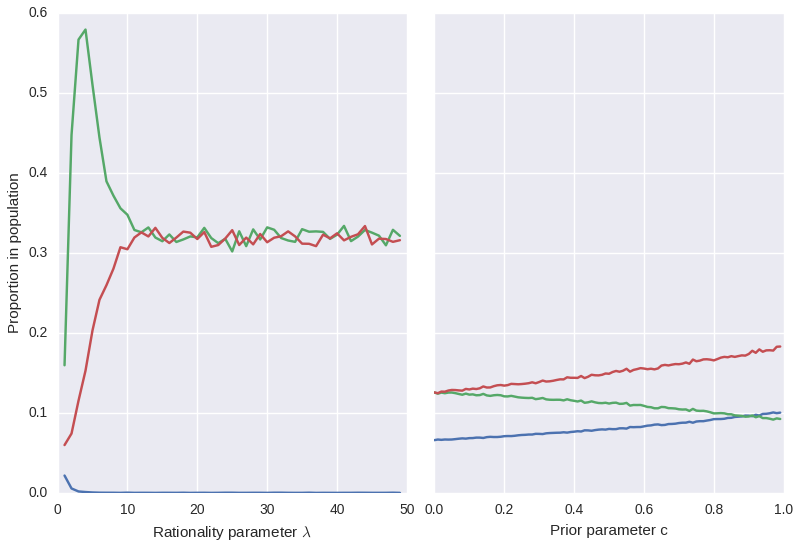
\includegraphics[scale=.5]{./only-R-or-M}
\caption{Mean proportions of target types after $20$ generations in $1000$ populations with only replication (A; $\alpha = 1$) and only mutation (B; $\alpha =1, \lambda = 30, k = 5$).}
\label{fig:either-R-or-M}
\end{figure}

\paragraph{Learnability only.} To get an impression of the effect of iterated learning without a pressure towards expressivity, we first consider (relatively) deterministic parental data production ($\lambda = 20, \alpha = 1$). In this way small data sequences suffice for learners to differentiate types that produce strongly diverging expressions. In line with \citeposs{griffiths+kalish:2007} analysis, under these conditions the resulting populations converge to the learner's prior distribution when sampling from the posterior. This is shown in the right-hand side of Figure \ref{fig:either-R-or-M}, which directly reflects the prior distribution for each value of $c$.

Inspecting the effects of these dynamics separately not only gives some intuitions about the parameters' influence, but also highlights some of their broader implications. First and foremost, neither dynamic comes close to converging to a monomorphic population under most parameter configurations. For instance, types using $L_4$ can come to occupy a large proportion of the final population. However, this holds only for a restricted range of low degrees of rationality. Apart from polymorphy, both dynamics make some undesirable predictions. A pressure only towards expressivity leads to the selection of types using $L_4$ to $L_6$ and to the ejection of $L_1$ to $L_3$. However, it can not explain the regular selection of $L_5$-like semantics over either of these functionally similar alternatives. In contrast, a pressure only towards learnability has a modest but clear effect in differentiating $L_5$ from these alternatives but fails to rule out functionally suboptimal types such as tautological $L_3$. This showcases that, while the bias plays a major role for the contrast between $L_4$ and $L_5$, on its own it does not enable types that fail to convey an upper-bound to establish themselves in the population. In sum, neither dynamic on its own is a suitable candidate to provide a justification for the predicted prevalence of $L_5$-like semantics. 

\paragraph{Expressivity and learnability.} Figure \ref{fig:cost} illustrates the effect of the learning bias after $20$ generations across values of $c$ with $l = 1$ (A) and $l =3$ (B). More detailed results for all types across a sample of $c$-values are presented in Table \ref{tab:numeric-results}. Overall, these results suggest that in the present setup a weak bias is sufficient to lead to a selection of $L_5$ over $L_4$. As in the simulations that only considered learnability, this effect increases with the bias' strength provided $L_5$ users are pragmatic. Importantly, the addition of a pressure towards expressivity magnifies this effect by dampening the proliferation of functionally suboptimal types advantaged by the learning bias. As stressed above, this suggests that neither the learning bias nor functional pressure alone but their combination lead to the systematic lack of semantic upper-bounds in scalar expressions.

\begin{figure}
\centering
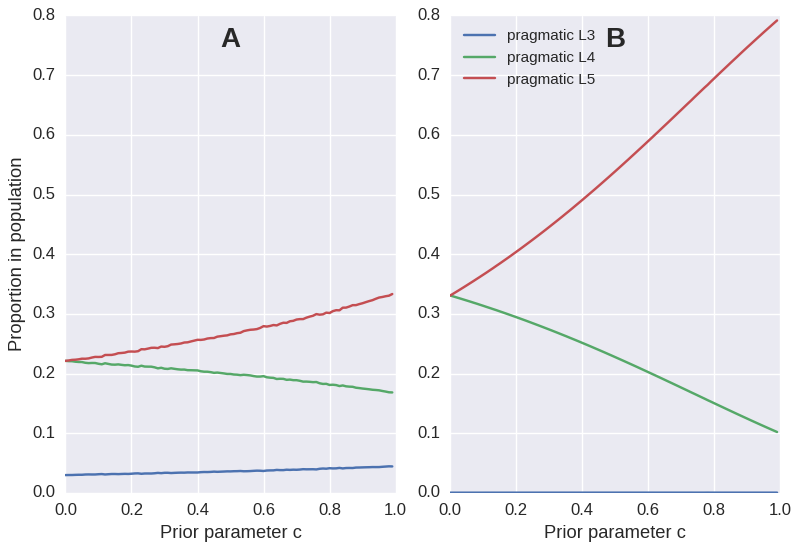
\includegraphics[scale=.5]{./fig2-rmd}
\label{fig:cost}
\caption{Mean proportions of target types after $20$ generations in $1000$ populations across bias values $c \in [0,1]$ with $l =1$ in A and $l = 3$ in B ($\alpha =1, \lambda = 20, k = 5$).}
\end{figure}


\begin{table}
\centering 
\begin{tabular}{l | c c c c c| c c c c c c c c}
\multicolumn{1}{c}{~} & \multicolumn{5}{c}{$l = 1$} & ~ & \multicolumn{5}{c}{$l = 10$}\\ \hline \hline
c  & 0 & .01 & .05 & .1 & .8 & ~ & 0 & .01 & .05 & .1 & .8\\ \hline \hline
lit. $L_1$& .03 & .03 & .03 & .03  & .04 & ~ & $\epsilon$ & $\epsilon$ & $\epsilon$ & $\epsilon$ & $\epsilon$\\ 
lit. $L_2$ & .03 & .03 & .03 & .03 & .01 & ~ & $\epsilon$& $\epsilon$ & $\epsilon$ & $\epsilon$ & $\epsilon$\\
lit. $L_3$ & .03 & .03 & .03 & .03 & .04 & ~ & $\epsilon$& $\epsilon$ & $\epsilon$ & $\epsilon$ & $\epsilon$\\
lit. $L_4$ & .07 & .07 & .07 & .07 & .06 & ~ & $\epsilon$& $\epsilon$ & $\epsilon$ & $\epsilon$ & $\epsilon$\\
lit. $L_5$ & .04 & .04 & .05 & .05 & .06& ~ & $\epsilon$& $\epsilon$ & $\epsilon$ & $\epsilon$ & $\epsilon$\\
lit. $L_6$ & .04 & .04 & .04 & .04 & .04& ~ & $\epsilon$& $\epsilon$ & $\epsilon$ & $\epsilon$ & $\epsilon$\\ \hline
prg. $L_1$ & .03 & .03 & .03 & .03 & .04& ~ & $\epsilon$& $\epsilon$ & $\epsilon$ & $\epsilon$ & $\epsilon$ \\
prg. $L_2$ & .03 & .03 & .03 & .03 & .01& ~ & $\epsilon$& $\epsilon$ & $\epsilon$ & $\epsilon$ & $\epsilon$ \\
prg. $L_3$ & .03 & .03 & .03 & .03 & .04& ~ & $\epsilon$& $\epsilon$ & $\epsilon$ & $\epsilon$ & $\epsilon$ \\ 
prg. $L_4$ & .22 & .22 & .22 & .22 & .18& ~ & .33& .33 & .32 & .31 & .15 \\
prg. $L_5$ & .22 & .22 & .22 & .23 & .3& ~ & .33& .33 & .35 & .37 & .7 \\
prg. $L_6$ & .22 & .22 & .22 & .22 & .18& ~ & .33& .33 & .32 & .31 & .15   
\end{tabular}
\caption{Mean proportions of types in $1000$ populations after $20$ generations across bias values $c \in [0,1]$ with $l =1$ and $l = 3$ ($\alpha = 1, \lambda = 30, k = 5$), $\epsilon < 0.005$}
\label{tab:numeric-results}
\end{table}

This data suggests that the proportion of scalar implicature users that is predicted primarily hinges on three aspects of the model. First, the degree to which linguistic behavior is deterministic, controlled by $\lambda$ and $\alpha$, plays a role both for expressivity as well as for producing data that allows learners to discriminate this type from others. Second, the learning bias $c$, leads learners to discriminate and prefer $L_5$ over $L_4$ and $L_5$. Lastly, the posterior parameter $l$ magnifies the effects of the learning bias in tandem with replication. This interaction is shown in \ref{fig:prior-posterior}. In the present setup posterior sampling can lead to the incumbency of pragmatic $L_5$, but not even a strong favorable learning bias manages to completely drive out competing types (cf. \ref{fig:cost}.A). However, as posterior maximization increases, the range of bias values within which this type takes over the population increases drastically. 

\hl{More  discussion about parameter interaction: changes in sequence length influence the population in a predictable way: smaller values lead to more heterogeneous populations whereas larger ones lead to more pronounced differences. This is expected insofar as the likelihood that a sequence of length $1$ was produced by any type is relatively uniform (modulo prior) whereas the likelihood of types with lexica $L_1$ - $L_3$ to produce, for instance, a sequence of $10$ observations consistently with the same state-message combination is less likely than for pragmatic players using $L_4$ - $L_6$ or literal $L_4$. Thus, while noteworthy, sequence length has no direct bearing on the main contrast of interest. Similar considerations hold for $\alpha$ and $\lambda$ -- set to $1$ and $50$ in the following. Overall, lower rationality in $\lambda$ or more pragmatic violations in $\alpha$ lead to a higher selection of lexica with semantic upper-bounds. The fitness of pragmatic behavior increases with higher $\lambda$-/$\alpha$-values. In other words, these parameters level the functional contrast between $L_4$ and $L_5$. }


\begin{figure}
\centering
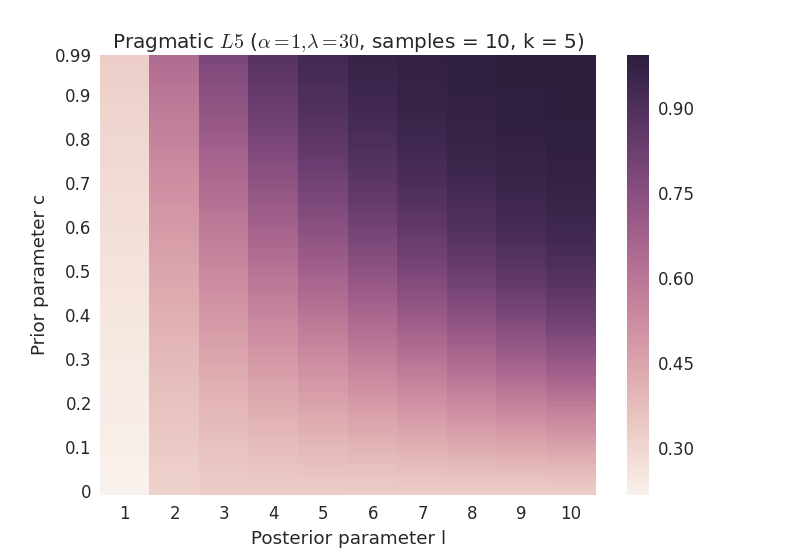
\includegraphics[scale=.5]{../presentations/01heatmap}
\caption{Mean proportion of pragmatic $L_5$ in $1000$ populations after $20$ generations ($\alpha = 1, \lambda = 30, k = 5$)}
\label{fig:prior-posterior}
\end{figure}



\subsection{Discussion}
Broadly speaking these results suggest that a lack of semantic upper-bounds coupled with pragmatic reasoning can overcome selective pressures and stabilize in a population provided there is a bias for simpler representations. This outcome is particularly encouraging in light of the other advantages a lack of semantic upper-bounds may confer that were discussed above. 
\hl{The model gives a justification for lexicalization patterns found in natural language, as well as for the failure to lexicalize certain pragmatic inferences. That is, while the puzzle raised by semantics is hard to explain by purely functionalmeans,  we  suggest  part  of  the  answer  to  lie  in  learnability.   Simpler semantic representations are more likely to be learned,  and pragmatic reasoning can counteract functional disadvantages otherwise incurred.  This result is of particular relevance for the longstanding assumption of a divide and interaction between semantics and pragmatics and offers an account of why (certain) pragmatic inferences are not part of the literal meaning of expressions. It furthermore leaves open the possibility of such inferences to fossilize when they do not compete against a lexical simplicity bias}

The model predicts this result to hinge on four conditions. First, types need to be pressured toward both expressivity and learnability. Second, language use can not be too unpredictable; low $\alpha$ or $\lambda$ values render non-upper-bounded lexical meanings more prone to communicative failure and more difficult to learn. Third, learners should prefer simpler over more complex lexical representations. Fourth, the strength by which they need to be preferred depends on the inferential mechanism of learners. That is, to which degree learners maximize the posterior. Put differently, high rationality in learning and choice requires a weaker bias towards simpler representations. The selection of lexical meanings lacking upper-bounds is robust against parameter perturbations under these conditions.

A large range of parameter values lead to the stable incumbency of scalar implicatures. However, while this is predicted by the literature, it is less clear to what proportion other types should be represented. On the one hand, there are  reasons to expect functionally suboptimal types $L_1$-$L_3$ to be largely ruled out. They fail to enable their users to communicate without substantial error both amongst themselves and with other types. In short, these lexica stand at odds with past theoretical and empirical observations. On the other, this is not so for $L_4$.\footnote{$L_6$ presents a special case. In our current setup, it mirrors $L_5$ in allowing for pragmatic strenghtening of message $m_2$ rather than $m_1$. However, its association of $s_1$ with $m_1$ and $s_2$ with $m_2$ under favourable parameter conditions is achieved by ruling out the ``some but not all''-state $s_1$ and not, as with scalar implicatures, the ``all''-state $s_2$. $L_6$ speakers thusly have a ``some''-message strengthened to convey ``all but not some but not all''. The observation that monomorphemic expression that lexically rule out stronger alternatives are unattested across languages has received substantial argumentative support (most prominently in \citealt[252-267]{horn:1984} but also e.g. in \citealt{horn:1972,traugott:2004,vdAuwera:2010}). However, our present setup is blind to these differences.} Notwithstanding, it is possible that natural language communities are composed of such mixed populations or that a single speaker may entertain $L_4$-like semantics for one scalar expression and $L_5$-like semantics for another \hl{CITATIONS FOR THIS PURPOSE}.   

Lastly, there are a number of extensions one may want to consider. For instance, the consideration of larger lexica that consider epistemic uncertainty. Another interesting additon relates to possible disadvantages of pragmatic reasoning and the effect of state frequencies on fossilization. We tacitly assumed pragmatic reasoning to come at no cost. However, there is experimental evidence that suggests  that the pragmatic derivation of upper-bounds costs effort and takes additional processing time (cf. \citealt{deNeys+schaeken:2007, huang+snedeker:2009}. This raises the question at which point such usage-based cost undercuts the learnability advantage of simpler semantic representations. As noted above, this might also depend on a given scalar expression and its frequency. Frequently drawn scalar implicatures might fossilize to avoid cost, while infrequent ones could still be computed on-line. 



\section{General discussion}
The model gives a justification for lexicalization patterns found in natural language, as well as for the failure to lexicalize certain pragmatic inferences. That is, while the puzzle raised by semantics is hard to explain by purely functional means, we suggest part of the answer to lie in learnability. Simpler semantic representations are more likely to be learned, and pragmatic reasoning can counteract functional disadvantages  otherwise incurred. This result is of particular relevance for the longstanding assumption of a divide and interaction between semantics and pragmatics and offers an account of why (certain) pragmatic inferences are not part of the literal meaning of expressions. It furthermore leaves open the possibility of such inferences to fossilize when they do not compete against a lexical simplicity bias.

A virtue of this model is that it allows for analysis specific modifications and extensions. Straightforward extensions include larger hypothesis spaces, as well as larger or different lexicon fragments. Another worthwhile modification relates to possible disadvantages of pragmatic reasoning. We tacitly assumed pragmatic reasoning to come at no cost. However, there is experimental evidence for the assumption that the pragmatic derivation of upper-bounds costs effort and takes additional processing time (cf. \citealt{deNeys+schaeken:2007, huang+snedeker:2009}). This raises the question at which point such usage-based cost undercuts the learnability advantage of simpler semantic representations.\footnote{In the present setup this modification has a straightforward effect: A penalty for pragmatic signaling lowers the fitness of pragmatic types, to the advantage of literal types. However, the penalty needs to be substantial to counteract the functional advantage pragmatic $L_5$ has over all but $L_4$ together with its learning advantage.}


The model combines:
\begin{itemize}
  \item game-theoretical models of functional pressure towards efficient communication
  \item effects of learning biases on (iterated) language learning
  \item assumptions about particular learning biases (Piantadosi et al. 20XX)
  \item probabilistic speaker and listener types of various pragmatic sophistication (Frank \& Goodman, 2012; Franke \& Jäger, 2014)
  \item speaker and listener types with different lexica (Bergen et al. 2012, to appear)
\end{itemize}

Discussion about expressivity as external to learning (cf. Stadler, replicator-papers by Kenny Smith, Kirby et al 2015). Possibly add appendix with direct comparison between IL and RMD.


\section{Conclusion}


\hl{The development of natural languages is driven by complex intertwined pressures. Drawing from past insights we put forward a model that allows for a general and malleable integration of core aspects involved in this process.  Chiefly, the model combines functional pressure, iterated Bayesian learning, and probabilistic speaker and hearer models.  In particular,  this analysis addresses longstanding issues concerning
the  semantics-pragmatics  divide.   It  shows  that  when  pressured for learnability and expressivity, the former force drives for simpler semantic representations inasmuch as pragmatics can compensate for them in language use.  Consequently, semantic  patterns  can  be  explained  in  virtue  of  the  linguistic behavior  of  their  users  and  their  complexity.   Furthermore, the ease of acquisition of simpler semantics offers an answer to why natural languages do not lexicalize certain pragmatic inferences.}

%%% Old snippets %%%
%\section{Conveying upper-bounds}
%Scalar inferences refer to the pragmatic derivation of an upper-bound for weak scalar expressions to the effect that stronger alternatives are inferred to not hold, e.g. {\em some students came} may be taken to convey that {\em not all students came}. The order of an expression such as {\em some} with respect to an alternative, e.g., {\em all}, is induced by entailment. For instance, {\em all students came} entails {\em most students came}, which in turn entails {\em some students came}. In this sense, {\em some} is weaker than {\em all}. A considerable class of natural language expressions do not lexicalize an upper-bound and can be ordered in this fashion, allowing for their pragmatic strengthening. As alluded at above, examples in English include numerals, scalar adjectives, quantifiers, modals, and connectives. \hl{possibly add some typological data on universality, frequency, monomorphemic status}
%
%The pragmatic enrichment of the semantic content of such expressions is enabled by mutual reasoning \citep{grice:1975}. More specifically, it is driven by interlocutors' mutual expectations of rational language use. The hearer reasons about the speaker's choice of a weak alternative over a stronger one. Had the speaker known that a stronger alternatives holds, she would have said so as this would have been more informative. Since she did not, the hearer can infer that the stronger alternative does not hold. Analogously, a speaker who reasons about her addressee may rely on her to derive this inference. In this way, a strengthened, upper-bounded, state of affairs can be conveyed without codifying the bound explicitly in the semantics.
%
%However, while pragmatics offers means to convey upper-bounds, the question why they are not part of the lexical meaning of these expressions remains. There are two main explanatory venues for this pattern. The first targets the functional advantages a lack of upper-bounds may confer to language users, whereas the second focuses on a learnability advantage of simpler over more complex semantic representations. 
%
%\paragraph{Function-based explanations.} Two assumptions are key to the pragmatic strengthening of weak alternatives: (the assumption of) cooperation and knowledge about the issue at hand. That is, the hearer needs to assume the speaker to be as informative as possible, i.e., not to withhold information, and that the speaker is knowlegeable, e.g., she knows whether {\em all students came}. Conversely, the speaker needs to assume the hearer to regard these conditions as satisfied. It is not difficult to imagine scenarios where either or both of these conditions are not given. For instance, the speaker may (be assumed to) not want to disclose all information about the students' attendance, or may have left early without being able to verify the attendance to a satisfactory degree. 
%
%\hl{Discussion of functional pressures for a lack of upper-bounds}

%\paragraph{Learning-based explanations.}
%
%\hl{Discussion of our main assumption that a lack of upper-bounds provides a learnability advantage framed in terms of relative representational simplicity over the codification of an upper-bound. {\bf Should this be made precise? If so, in which way?}}

%\bibliographystyle{apacite}
\bibliographystyle{unsrtnat}

%\setlength{\bibleftmargin}{.125in}
%\setlength{\bibindent}{-\bibleftmargin}
\bibliography{./bounds-rmd}


\end{document}
